\chapter{Geração de gráficos}
\label{cap7}

Para proceder à análise dos dados, é necessário que os dados sejam organizados num formato que permita a leitura e a visualização dos dados facilitada a humanos. Foram gerados os gráficos para a análise de \textit{sentiments} e \textit{keywords} em \textit{sets} de totais e de forma temporal.

Para os gráficos de totais, foi utilizado o pacote \textit{matplotlib} \cite{va1} e o \textit{WordCloud} \cite{gfg3} em que foram usados todos os dados disponíveis (das três plataformas). Já os gráficos de análises temporais foram gerados apenas com os dados do \textit{TripAdvisor}, visto que não só eram os mais completos e extensos de todas as categorias de estabelecimento, como também foi possível extrair as datas de criação dos \textit{reviews}.

\section{Gráficos de totais}

Com gráficos de totais, queremos dizer que nos dados apresentados e nas análises não é considerado o desenvolvimento temporal, mas sim o desenvolvimento de um total de \textit{reviews}, ou seja, o mês e ano são descartados.

\section{Metodologia}

Para a geração dos gráficos de totais, foi utilizado o pacote \textit{matplotlib} \cite{va1} e o \textit{wordcloud} \cite{gfg3} num \textit{script Python}, que iterava sobre os dados disponíveis e gerava os gráficos para cada estabelecimento.

Os tipos de gráficos gerados são: gráficos circulares de \textit{sentiments}, gráficos de \textit{keywords} e nuvens de \textit{keywords}. Os quais demonstram a quantidade de \textit{sentiments} positivos e negativos, as dez \textit{keywords} mais frequentes e as nuvens de \textit{keywords} limitadas até cem palavras.

\subsection{Execução}

Para cada tipo de estabelecimento, de cada plataforma, foi accionada as rotinas de geração dos gráficos. As quais foram exportadas em formato de imagem. Iterando sobre os tipos de estabelecimento e as plataformas, em que itera sobre os dados disponíveis, segmentados em \textit{sentiments} e \textit{keywords}, que passam por uma e duas funções respectivamente. Gerando e exportando \textit{.jpg} dos gráficos e nuvens.

\subsection{Resultados}

Como se podem verificar nestas três imagens (figura: \cite{fig:exemplofig21sentimentsTrip},  figura: \cite{fig:exemplofig21keywordsTrip}, figura: \cite{fig:exemplofig21cloudTrip}), os gráficos de totais apresentam um desenvolvimento de \textit{sentiments} e \textit{keywords}, que demonstra um \textit{sentiment} total positivo no nosso turismo, e \textit{keywords} que apresentam a satisfação com o serviço ou uma característica do estabelecimento.

\begin{figure}[!htb]
\centering
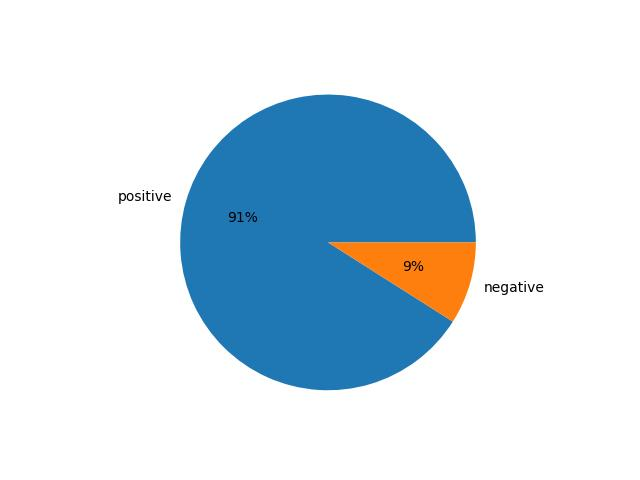
\includegraphics[width=7cm]{figuras/TripAdvisor/Hotels/hotel21_sentiments.jpeg}
\caption{Gráfico circular gerado baseando-se nos \textit{sentiments} dados da plataforma \textit{TripAdvisor} referente à Herdade das Barradas da Serra}
\label{fig:exemplofig21sentimentsTrip}
\end{figure}

\begin{figure}[!htb]
\centering
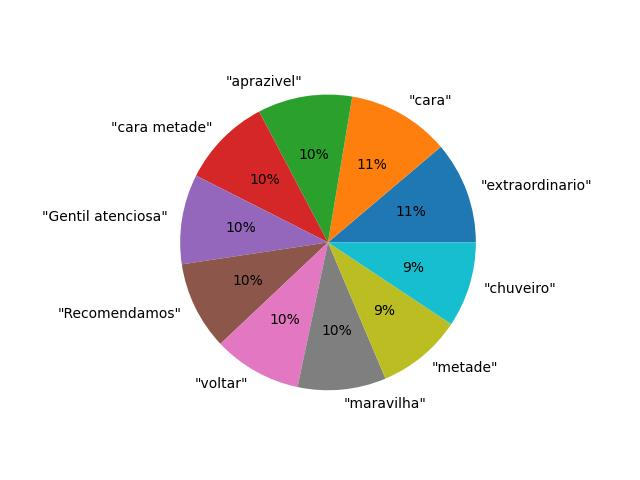
\includegraphics[width=7cm]{figuras/TripAdvisor/Hotels/hotel21_keywords.jpeg}
\caption{Gráfico circular gerado baseando-se nas \textit{keywords} mais usadas da plataforma \textit{TripAdvisor} referente à Herdade das Barradas da Serra}
\label{fig:exemplofig21keywordsTrip}
\end{figure}

\begin{figure}[!htb]
\centering
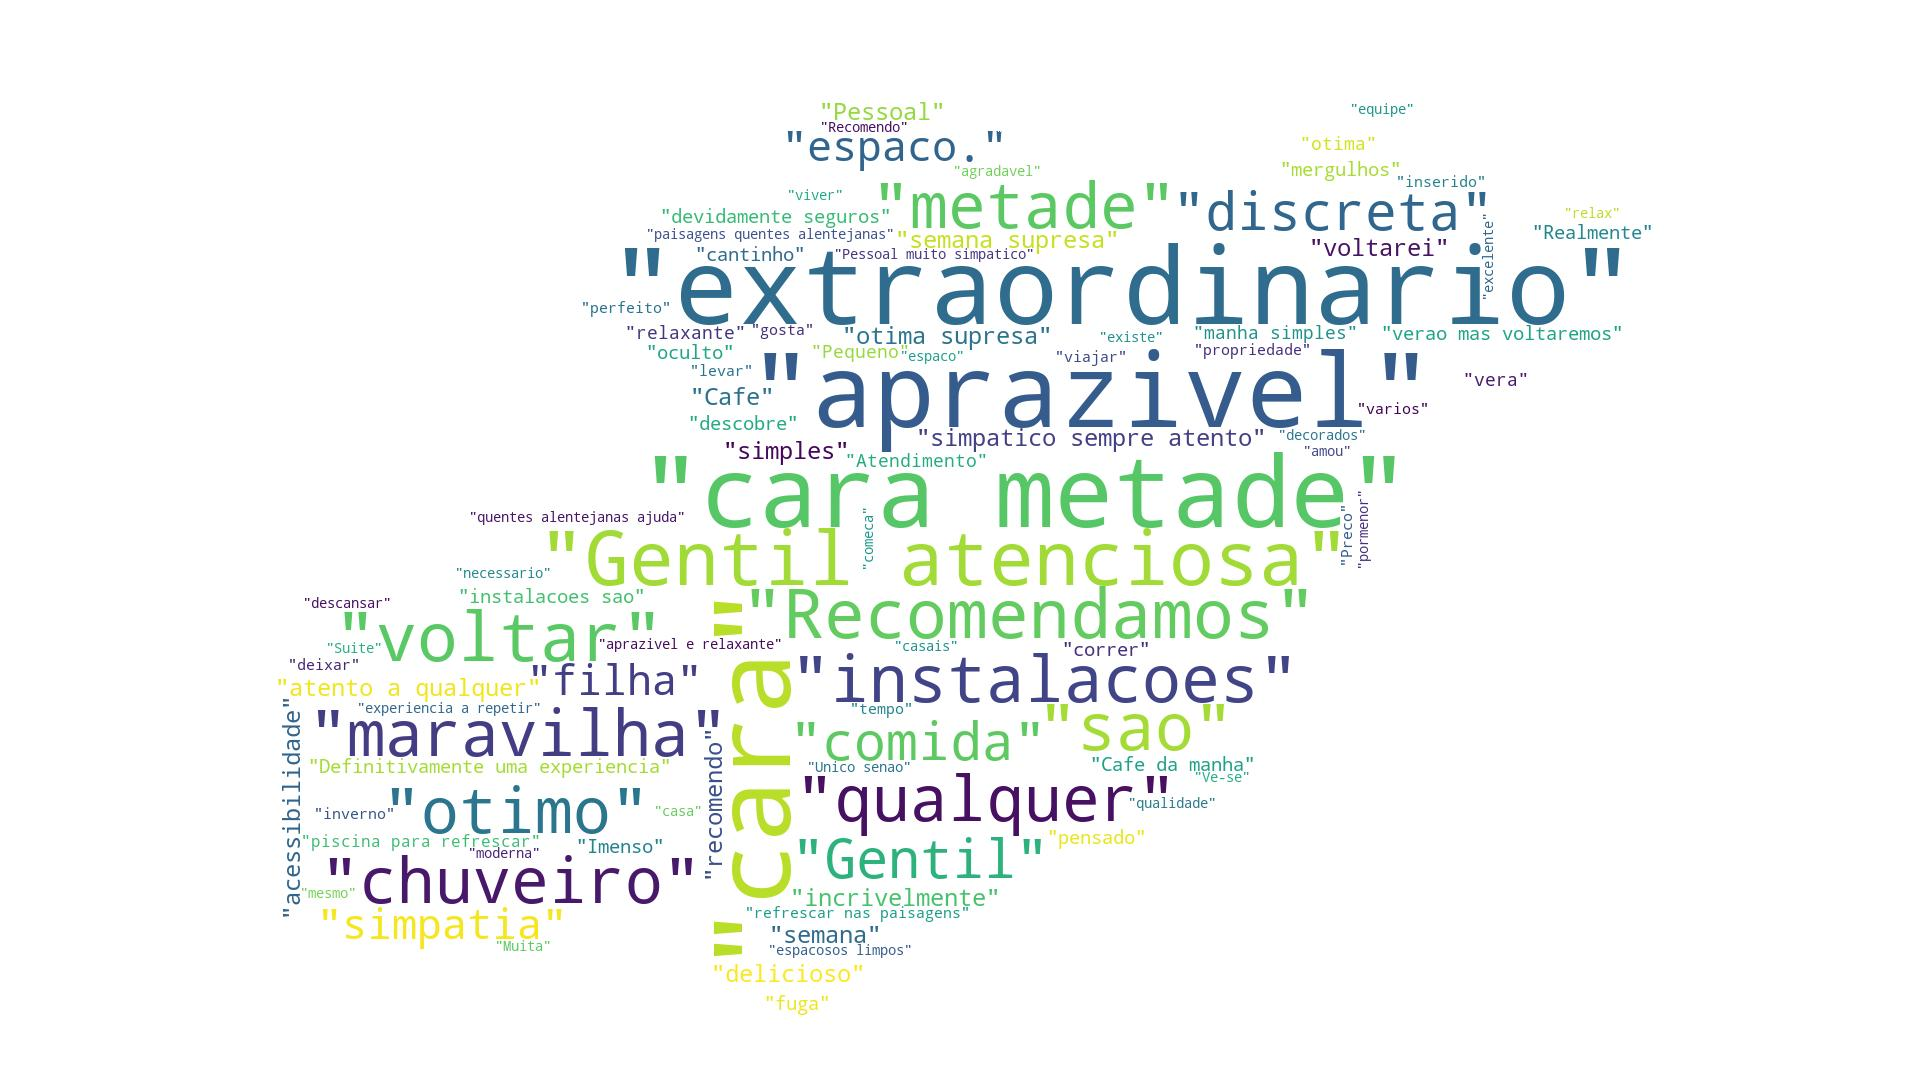
\includegraphics[width=7cm]{figuras/TripAdvisor/Hotels/hotel21_keywordcloud.jpeg}
\caption{Gráfico de \textit{keywords} e nuvens de \textit{keywords} contendo as \textit{keywords} mais usadas da plataforma \textit{TripAdvisor} referente à Herdade das Barradas da Serra}
\label{fig:exemplofig21cloudTrip}
\end{figure}


\section{Gráficos temporais}

Com gráficos temporais, queremos dizer que nos dados apresentados e nas análises é considerado o desenvolvimento temporal, quer isto dizer que as \textit{reviews} mostradas ao longo do tempo tornam possível verificar as datas em que foram escritas e a quantidade que cada hotel/restaurante/atracção recebeu ao longo dos anos e meses.

\subsection{Metodologia}

Para a geração dos gráficos temporais, foi utilizado o \textit{software PowerBI}, que utilizava os ficheiros .csv gerados e organizados previamente vindos da base de dados, contendo todas as informações em ficheiros únicos.
Os gráficos gerados são: gráficos circulares e de tabelas. Os quais demonstram a quantidade de \textit{sentiments} e \textit{keywords} usadas ao longo do tempo por cada hotel, divididos por anos e meses e também por cada hotel.

\subsection{Execução}

Os ficheiros \textit{.csv} que contêm as informações relativas a todas as \textit{keywords} e \textit{sentiments}, foram importados para o \textit{software PowerBI} e posteriormente organizados da maneira que o grupo achou mais conveniente para que os gráficos ficassem o mais apresentáveis e visivelmente mais fáceis para analisar os dados. Posteriormente os gráficos circulares e de tabelas foram exportados para \textit{.jpg} e guardados. 

\subsection{Resultados}

Como se podem verificar nestas três imagens (figura: \cite{fig:exemplofigqntsntmyear},  figura: \cite{fig:exemplofigqntyearbus}, figura: \cite{fig:exemplofigposneg}), os gráficos temporais apresentam um desenvolvimento de \textit{sentiments} e \textit{keywords} ao longo do tempo bastante positivo revelando-se um óptimo ponto para o nosso turismo e \textit{keywords} que mostram bastante agrado. 

\begin{figure}[!htb]
\centering
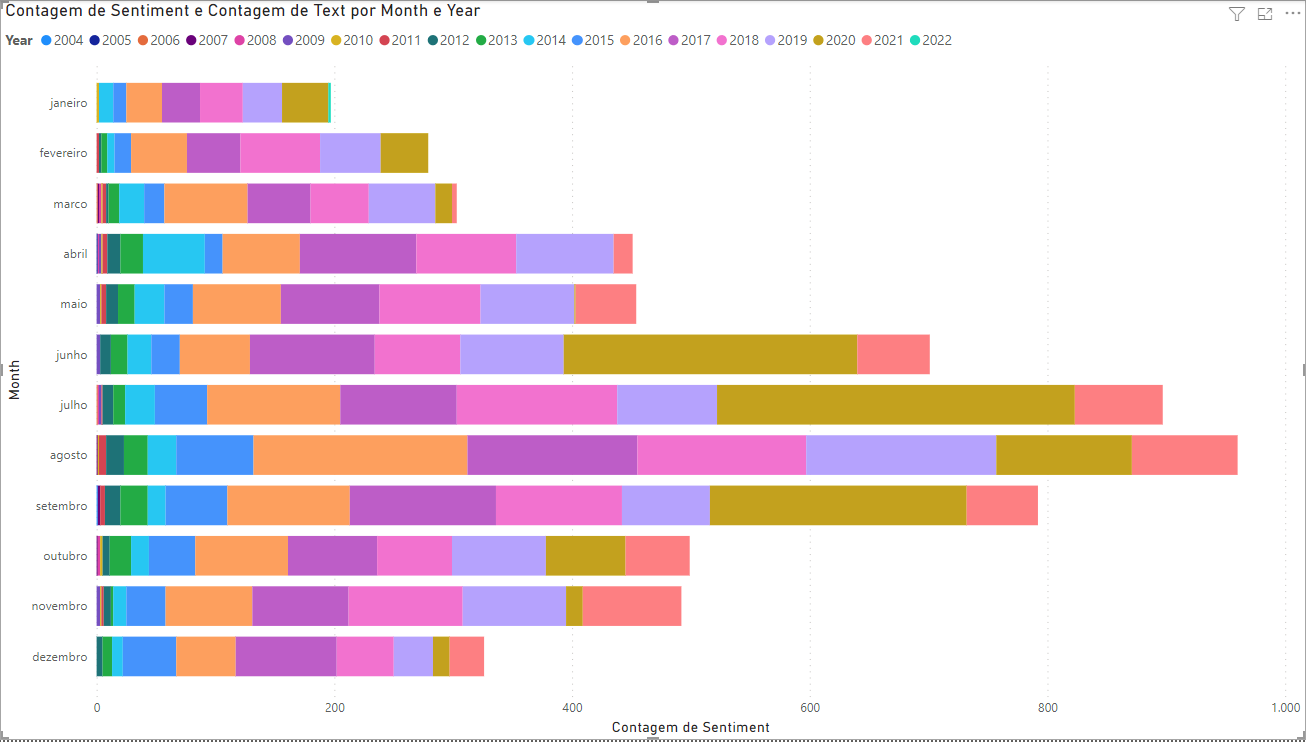
\includegraphics[width=7cm]{figuras/NrReviewsPerYear/TableGraph6.PNG}
\caption{Gráfico de tabelas gerado baseando-se em todos os \textit{sentiments} dados da plataforma \textit{TripAdvisor} ao longo dos anos}
\label{fig:exemplofigqntsntmyear}
\end{figure}

\begin{figure}[!htb]
\centering
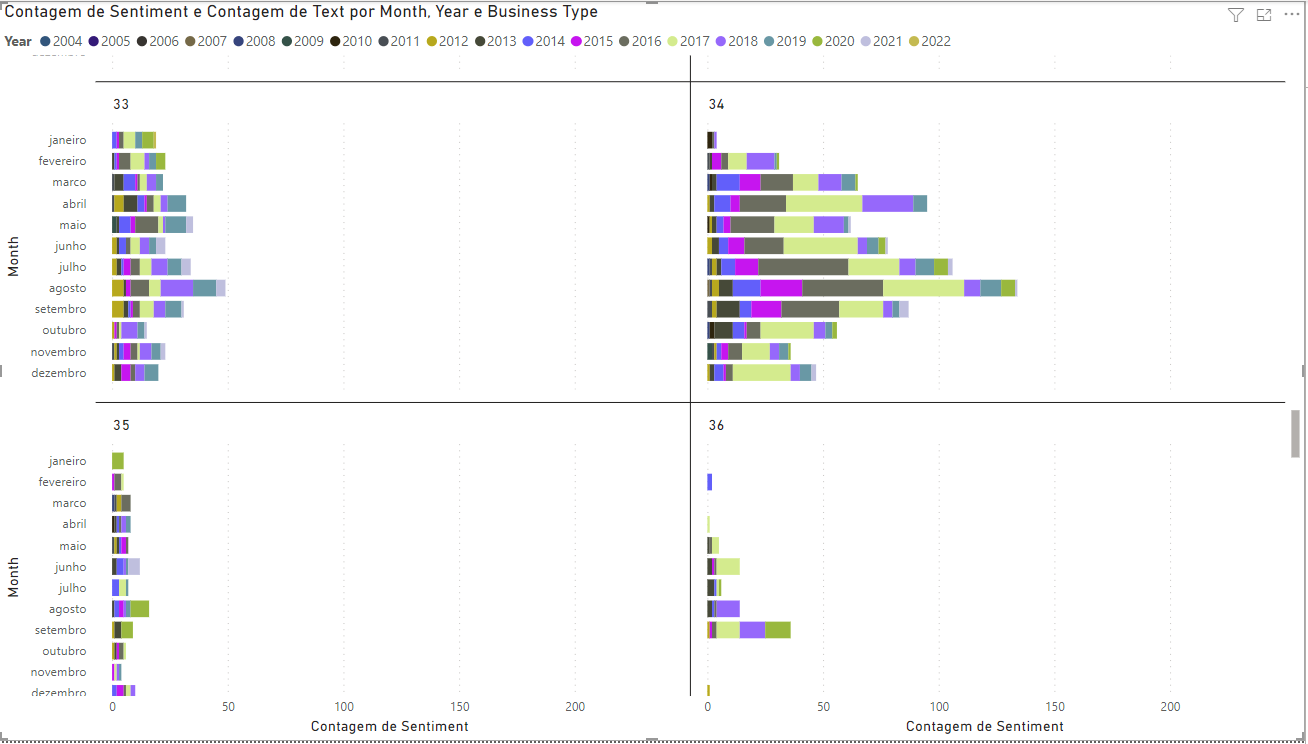
\includegraphics[width=7cm]{figuras/NrReviewsPerYear&BusinessType/8.PNG}
\caption{Gráfico de tabelas gerado baseando-se em todos os \textit{sentiments} da plataforma \textit{TripAdvisor} referente a cada hotel com o decorrer dos anos}
\label{fig:exemplofigqntyearbus}
\end{figure}

\begin{figure}[!htb]
\centering
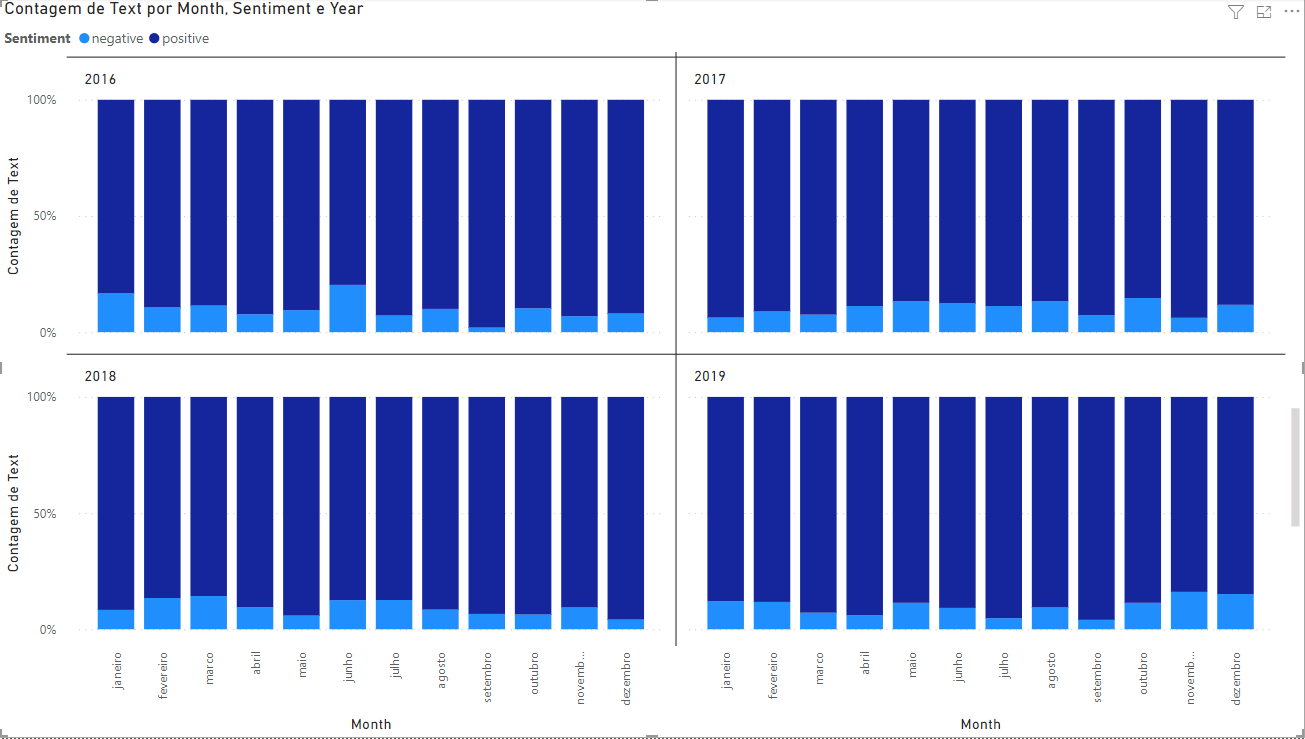
\includegraphics[width=7cm]{figuras/Pos&NegSentiments/TableGraph4.PNG}
\caption{Gráfico de tabelas gerado baseando-se na quantidade de \textit{sentiments} da plataforma \textit{TripAdvisor} positivos e negativos ao longo do tempo para cada hotel}
\label{fig:exemplofigposneg}
\end{figure}